%%%%%%%%%%%%%%%%%%%%%%%%%%%%%%%%%%%%%%%%%%%%%%%%%%%%%%%%%%%%%%%%%%%
%
% This is a general template file for the LaTeX package SVJour3
% for Springer journals.          Springer Heidelberg 2010/09/16
%
% Copy it to a new file with a new name and use it as the basis
% for your article. Delete % signs as needed.
%
% This template includes a few options for different layouts and
% content for various journals. Please consult a previous issue of
% your journal as needed.
%
%%%%%%%%%%%%%%%%%%%%%%%%%%%%%%%%%%%%%%%%%%%%%%%%%%%%%%%%%%%%%%%%%%%
%
\RequirePackage{fix-cm}
%
\documentclass[twocolumn]{svjour3}
%
\smartqed
%
\usepackage{graphicx}
\usepackage{hyperref}
\usepackage[round, sort&compress, numbers]{natbib}
\usepackage{multirow}
\usepackage{graphicx}
\usepackage{units}
\usepackage{color}
\usepackage{xspace}
%
\DeclareRobustCommand\IPCClongname{}
%
% please place your own definitions here and don't use \def but \newcommand{}{}
\newcommand{\pmlib}{\texttt{pmlib}\xspace}
%
% Insert the name of "your journal" with
% \journalname{myjournal}
%
\begin{document}

\title{Evaluating the Performance  and Energy Efficiency of COSMO-ART,
  a Coupled Numerical Weather Forecast and Chemical Transport Model}
% \thanks{This work was supported by the EU Project FP7 318793 ``EXA2GREEN''}}
%\subtitle{Write here subtitle}

%\titlerunning{Short form of title} % if too long for running head

\author{Joseph~Charles  \and William~Sawyer  \and  Manuel~F.~Dolz \and
  Cristiano~Malossi}

%\authorrunning{Short form of author list} % if too long for running
%head

\institute{J.~Charles, W.~Sawyer 
	\at Swiss National Supercomputing Centre (CSCS)
	\\ CH-6900 Lugano, Switzerland  
	%\\ Tel: +41  (0) 91  610 8216
 	\\ E-mails:~{\{joseph.charles,william.sawyer\}@cscs.ch} 
        \and M.~F.~Dolz 
        \at Dept. of Informatics, University of Hamburg
	\\ D-22.527 Hamburg, Germany
        %\\ Tel: +49 (0) 40 460094-404
        \\ \email{manuel.dolz@informatik.uni-hamburg.de}  
        \and C.~Malossi  
        \at IBM Zurich Research Laboratory 
        \\  CH-8000 Zurich, Switzerland
        %\\  Tel: +41 (0) 44 724 8616
        \\ \email{ACM@zurich.ibm.com}}

\date{Received: date / Accepted: date} % The correct dates will be
                                       % entered by the editor

\maketitle

\begin{abstract}
  In this paper we present  COSMO-ART, an extension of the operational
  weather  forecast  model  of   the  German  weather  service  (DWD),
  developed for  the evaluation of the interactions  of reactive gases
  and aerosol particles  with the state of atmosphere  at the regional
  scale. It  includes secondary aerosols,  directly emitted components
  like  soot,  mineral  dust,  sea  salt and  biological  material  as
  pollen. Processes such  as emissions, coagulation, condensation, dry
  deposition,  wet removal,  and sedimentation  of aerosols  are taken
  into account.   The overall performance  of this application  on HPC
  systems is analysed  by a profiling study to  determine hotspots and
  identify critical paths.   Moreover, we describe measurement devices
  and  energy-aware   techniques  employed  to   evaluate  the  energy
  footprint of the considered application and to get detailed insights
  about power bottlenecks.  Our motivation is to improve corresponding
  code   sections  to  sustain   high  performance   while  minimizing
  energy-to-solution.   This  preliminary  work  sets  the  basis  for
  subsequent studies to tackle  challenges related to energy efficient
  high performance computing in the framework of the Exa2Green project
  (\url{http://exa2green.eu/}).

\keywords{High performance computing  \and Energy-aware computing \and
  Green computing  \and Numerical weather  prediction \and Atmospheric
  chemistry  \and  Aerosols  modelling  \and  Profiling  methods  \and
  Benchmark analysis \and COSMO-ART coupled model}
% \PACS{PACS code1 \and PACS code2 \and more}
% \subclass{MSC code1 \and MSC code2 \and more}
\end{abstract}

\section{Introduction}
\label{intro}
The  interaction  between aerosols  and  clouds  presents  one of  the
biggest  uncertainties  in   present  day  climate  simulations.   The
chemistry involved is complex,  but there is a concerted international
effort to model the underlying processes through models. These models,
such as  the Aerosol  Reactive Transport (ART),  developed at  the KIT
(Karlsruhe  Institute of  Technology)  , offer  a  key opportunity  to
reduce   the  climate  uncertainty,   particularly  on   the  regional
scale. These  models can be coupled  with climate models,  such as the
regional  weather  and   climate  COSMO  (Consortium  for  Small-scale
Modelling) model  developed by the German Weather  Service (DWD).  The
COSMO model  is a weather forecast  model which has  become a standard
all  over Europe.   Beside the  federal weather  forecast  stations in
Germany  (Deutscher  Wetterdienst,  DWD),  Switzerland  (MeteoSchweiz,
MCH),  Italy (Ufficio  Generale  Spazio Aereo  e Meteorologia,  USAM),
Greece  (Hellenic   National  Meteorological  Service,   HNMS)  Poland
(Institute  of   Meteorology  and  Water   Management,  IMGW)  Romania
(National  Meteorological  Administration,  NMA) and  Russia  (Federal
Service for Hydrometeorology  and Environmental Monitoring, RHM), also
a   large  number   of  agencies   including  military   and  research
institutions  base their  forecasts on  COSMO. The  combined COSMO-ART
model is capable of simulating  aerosol distributions as well as their
interactions over Europe as well as other regional domains.

It has  been a major  scientific achievement to effectively  model the
underlying  chemical  processes   through  these  applications.   This
achievement  now   needs  to  be  fostered  by   reducing  its  energy
expense. Currently, resource allocation  is one of the key limitations
to scientists  in running the simulation periods  and resolutions they
would like.


\section{The COSMO-ART model system}
\label{sec:1}
\subsection{Model description}
\label{subsec:1.1}

COSMO-ART  (ART   stands  for  Aerosols  and   Reactive  Trace  gases,
\citealp{Vogel-2009}),  developed  at KIT  Karlsruhe  (Germany), is  a
regional  to  continental scale  model  coupled  online  to the  COSMO
numerical    weather    prediction    (NWP)    and    climate    model
\citep{Baldauf-2011}. COSMO is used  by several European countries for
operational weather  forecast. The  gaseous chemistry in  COSMO-ART is
solved by  a modified version  of the Regional Acid  Deposition Model,
Version  2 (RADM2)  mechanism \citep{Stockwell-1990},  which  has been
extended   to    describe   secondary   organic    aerosol   formation
\citep{Schell-2001, Athanasopoulou-2013} and hydroxyl recycling due to
isoprene chemistry \citep{Geiger-2003}  and heterogeneous reactions as
hydrolysis  of N2O5.  Aerosols are  represented by  the  modal aerosol
module MADE \citep{Ackermann-1998},  improved by explicit treatment of
soot aging  through condensation of  inorganic \citep{Riemer-2003} and
organic substances (MADEsoot).

The  five modes that  represent the  aerosol population  contain: pure
soot, secondary mixtures of sulfates, nitrates, ammonium, organics and
water (nucleation  and accumulation) and the internal  mixtures of all
these species in  both modes. Separate fine and  coarse emission modes
for  sea-salt,  dust  \citep{Stanelle-2010},  and  rest  anthropogenic
species  are treated by  six additional  modes.  Specific  modules are
included    to   simulate    the   dispersion    of    pollen   grains
\citep{Vogel-2008}   and  other  biological   particles.   Meteorology
affected emissions are also online coupled within the model system.

\subsection{Model setup}
\label{subsec:1.2}


\section{Experimental setup}
\label{sec:2}
\input{Sec2:Experimental-setup.tex}

\section{Evaluation}
\label{sec:3}
\subsection{Sofware environment}
\label{subsec:3.1}
The software environment on Monch  and Pilatus is controlled using the
modules framework which gives an easy and flexible mechanism to access
to all of the CSCS  provided compilers, tools and applications.  It is
particularly  useful for  testing code  portability  between different
compilers  or for  changing  between different  versions  of the  same
compiler.  INT2LM  and the COSMO-ART model are  implemented in Fortran
90 for distributed memory parallel computers using the Message Passing
Interface (MPI).  For  our initial benchmarking, we opted  for the GNU
compiler  (gcc/4.8.1 on  Monch,  gcc/4.8.2 on  Pilatus)  with the  -O3
compiler flag as  it generally gives a good  level of optimization and
the code runs faster in this configuration than when compiled with the
intel compiler  (intel/14.0.1), also available on  Monch.  Besides, we
installed the  MPICH2 implementation of MPI (mvapich2/1.9)  as well as
the  commonly  used   HDF5  (hdf5/1.8.12)  and  NetCDF  (netcdf/4.3.1)
libraries in favor of the  traditional GRIB library for the management
of  extremely  large and  complex  data  collections.   Note that  all
compute  nodes of  Monch  and Pilatus  used  respectively the  ``Linux
2.6.32-358.11.1.el6.x86\_64''   and   ``Linux   3.0.101-0.15-default''
operating systems.

\subsection{Run configuration}
\label{subsec:3.2}
The COSMO-ART model uses NAMELIST-input to specify runtime parameters
splitted into several groups:

\begin{itemize}
\item LMGRID: specifying the domain and the size of the grid,
\item RUNCTL: parameters for the model run,
\item TUNING: parameters for tuning physics and dynamics,
\item DYNCTL: parameters for the adiabatic model,
\item PHYCTL: parameters for the diabatic model,
\item COSMO\_ART: parameters for gases and aerosols model,
\item DIACTL: parameters for the diagnostic calculations,
\item SATCTL: controlling computation of synthetic satellite images,
\item IOCTL: controlling the I/O environment,
\item GRIBIN: controlling the grib input,
\item GRIBOUT: controlling the grib output,
\end{itemize}

\noindent
To run COSMO-ART the following input data are necessary:
\begin{itemize}
\item  Gas phase:  Anthropogenic emissions  for different  species and
  land use data for biogenic emissions and deposition,
\item Aerosol particles: Anthropogenic emissions,
\item Mineral dust: Soil specific land use data.
\end{itemize}

A snapshot of the code, which includes, at least conceptually, all the
information needed  to reproduce the  energy-to-solution benchmarks of
COSMO-ART, was  produced and run on a  full rack of 52  nodes on Monch
(monchc[029-080]), i.e.  a total of 1040 cores using 20 tasks per node
and on  a full rack of  42 nodes on Pilatus  (pilatus[03-44]), i.e.  a
total of  1344 cores using 16  tasks per node.   The calculated region
was  mapped to  the participating  processors using  a 2D-partitioning
strategy.  The distribution along the  x and y coordinates was defined
by setting: $nprocx=40$ and  $nprocy=26$ for Monch and $nprocx=28$ and
$nprocy=24$.  Besides as this version of COSMO-ART doesn't make use of
the   GRIB   library,  we   specified   $nprocio=0$   for  GRIB   I/O.
Hyperthreading is not considered in this study as previous attempts of
its use revealed that it always led to higher energy-to-solution.\\

Multiple production runs of COSMO-ART were performed to illustrate the
reproducibility  of   the  baseline,  and   quantify  the  significant
uncertainties in  the power measurement, as dictated  by the available
technology (see subsection~\ref{subsec:2.2}).

\subsection{Power-measurement results}
\label{subsec:3.3}
Measuring  the power  consumption on  one entire  Cray cabinet  is the
easiest    way    to    calculate   energy-to-solution    for    given
applications.  The total  energy  to solution  is the  straightforward
calculation:\\

Energy-to-solution  =  Integral  of  power consumption  over  the  job
duration\\

However, the average power consumption times the job duration is often
sufficient.

\subsubsection{Monch (CSCS - ETH Zurich)}
\begin{figure*}
  \includegraphics[width=0.4\textwidth]{Figs/NRJ_benchmark_Monch.eps}
  \caption{Isola E1 Rack 2 Total Power and Isola E1 Total Power}
  \label{fig:1}
\end{figure*}

The 1-day simulation was issued successfully twice, the start time and
execution time for both runs are:
\begin{itemize}
\item start=12:51:03, end=13:20:46 $\Rightarrow$ T = 00:29:43 = 1783 s
\item start=14:28:40, end=14:58:02 $\Rightarrow$ T = 00:29:22 = 1762 s
\end{itemize}

The power  consumption for  both jobs is  calculated by  averaging the
corresponding power  measurements from the Excel  file.  Power results
account for the  Isola E1 Rack 2 Total Power. As  time resolution is 5
minutes  for the  output  results, the  average  power consumption  is
computed   by  considering  6   values  for   each  single   run  (see
Table~\ref{tab:1}).

\begin{table}
  \begin{center}
    \caption{}
    \label{tab:1}
    \begin{tabular}{lll}
      \hline\noalign{\smallskip}
      Time & Measured power (W) & Average power (W)  \\
      \noalign{\smallskip}\hline\noalign{\smallskip}
      12:55:00 & 1.2355833333e+04 & 1.265852278e+04 \\ 
      13:00:00 & 1.2820266667e+04 &  \\
      13:05:00 & 1.2600743333e+04 &  \\ 
      13:10:00 & 1.2811580000e+04 &  \\
      13:15:00 & 1.2609680000e+04 &  \\
      13:20:00 & 1.2753033333e+04 &  \\
      \noalign{\smallskip}\hline\noalign{\smallskip}
      14:30:00 & 1.2019266667e+04 & 1.258640833e+04 \\ 
      14:35:00 & 1.2632253333e+04 &  \\
      14:40:00 & 1.2779040000e+04 &  \\
      14:45:00 & 1.2753180000e+04 &  \\
      14:50:00 & 1.2610476667e+04 &  \\
      14:55:00 & 1.2724233333e+04 &  \\
      \noalign{\smallskip}\hline
    \end{tabular}
  \end{center}
\end{table}

Thus, the total energy consumption corresponds to: 
\begin{itemize}
\item E  = 1783 x 12658.52278  = 22570146.11674 J $\sim$  22.57 MJ per
  day of simulation
\item E  = 1762 x 12586.40833  = 22177251.47746 J $\sim$  22.18 MJ per
  day of simulation
\end{itemize}

\subsubsection{Pilatus (CSCS - ETH Zurich)}
\begin{figure*}
  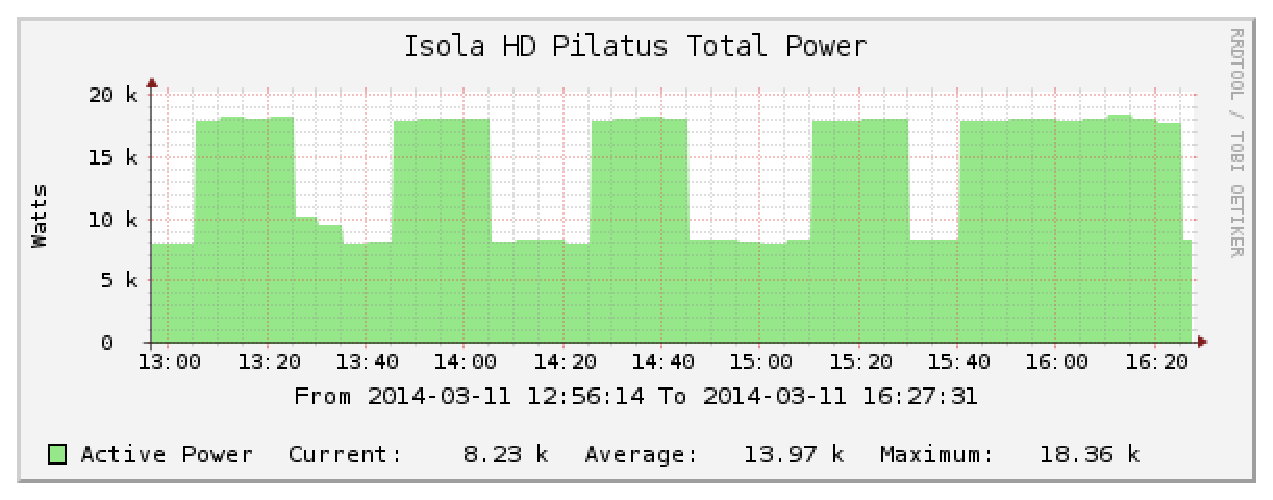
\includegraphics[width=0.4\textwidth]{Figs/NRJ_benchmark_Pilatus.eps}
  \caption{Isola HD Pilatus Total Power}
  \label{fig:2}
\end{figure*}

The 1-day simulation was issued successfully four times and the 2-days
run only once, the start time and execution time for all jobs are:
\begin{itemize}
\item start=13:07:25, end=13:29:47 $\Rightarrow$ T = 00:22:22 = 1342 s
\item start=13:46:04, end=14:08:30 $\Rightarrow$ T = 00:22:26 = 1346 s
\item start=14:27:51, end=14:50:01 $\Rightarrow$ T = 00:22:10 = 1330 s
\item start=15:10:04, end=15:32:17 $\Rightarrow$ T = 00:22:13 = 1333 s
\item start=15:41:48, end=16:26:13 $\Rightarrow$ T = 00:44:25 = 2665 s
\end{itemize}

Again, the power  consumption for all jobs is  calculated by averaging
the  corresponding  power  measurements  from the  Excel  file.  Power
results  account  for  the  Isola  HD Pilatus  Total  Power.  As  time
resolution  is 5  minutes for  the output  results, the  average power
consumption is computed by considering  4 values for each single 1-day
run and 9 values for the 2-days run (see Table~\ref{tab:2}).

\begin{table}
  \begin{center}
    \caption{}
    \label{tab:2}
    \begin{tabular}{lll}
      \hline\noalign{\smallskip}
      Time & Measured power (W) & Average power (W)  \\
      \noalign{\smallskip}\hline\noalign{\smallskip}
       13:10:00 & 1.7824080000e+04 & 1.812201417e+04 \\ 
       13:15:00 & 1.8293650000e+04 &  \\ 
       13:20:00 & 1.8125140000e+04 &  \\ 
       13:25:00 & 1.8245186667e+04 &  \\ 
      \noalign{\smallskip}\hline\noalign{\smallskip}
       13:50:00 & 1.7849206667e+04 & 1.797961083e+04 \\ 
       13:55:00 & 1.7977790000e+04 &  \\ 
       14:00:00 & 1.8030646667e+04 &  \\ 
       14:05:00 & 1.8060800000e+04 &  \\ 
      \noalign{\smallskip}\hline\noalign{\smallskip}
       14:30:00 & 1.7868826667e+04 & 1.806545167e+04 \\ 
       14:35:00 & 1.8115786667e+04 &  \\ 
       14:40:00 & 1.8188520000e+04 &  \\ 
       14:45:00 & 1.8088673333e+04 &  \\ 
      \noalign{\smallskip}\hline\noalign{\smallskip}
       15:15:00 & 1.7857800000e+04 & 1.797302833e+04 \\ 
       15:20:00 & 1.7962513333e+04 &  \\ 
       15:25:00 & 1.8078226667e+04 &  \\ 
       15:30:00 & 1.7993573333e+04 &  \\ 
      \noalign{\smallskip}\hline\noalign{\smallskip}
       15:45:00 & 1.7801980000e+04 & 1.799757815e+04 \\ 
       15:50:00 & 1.7925386667e+04 &  \\ 
       15:55:00 & 1.8076986667e+04 &  \\ 
       16:00:00 & 1.8082966667e+04 &  \\ 
       16:05:00 & 1.7903206667e+04 &  \\ 
       16:10:00 & 1.8063913333e+04 &  \\ 
       16:15:00 & 1.8355030000e+04 &  \\ 
       16:20:00 & 1.7971580000e+04 &  \\ 
       16:25:00 & 1.7797153333e+04 &  \\ 
      \noalign{\smallskip}\hline
    \end{tabular}
  \end{center}
\end{table}

Thus, the total energy consumption corresponds to: 
\begin{itemize}
\item E = 1342 x 18122.01417 = 24319743.01614 J $\sim$ 24.32 MJ per day of simulation
\item E = 1346 x 17979.61083 = 24200556.17718 J $\sim$ 24.20 MJ per day of simulation
\item E = 1330 x 18065.45167 = 24027050.72110 J $\sim$ 24.03 MJ per day of simulation
\item E = 1333 x 17973.02833 = 23958046.76389 J $\sim$ 23.96 MJ per day of simulation
\item E = 2665 x 17997.57815 = 47963545.76975 J $\sim$ 47.96 MJ per day of simulation
\end{itemize}


\section{Related work}
\label{sec:4}
\input{Sec4:Related.tex}

\section{Conclusion}
\label{concl}
We  have   presented  a  methodology  for   comparing  performance  of
COSMO-ART,  a  regional  weather  forecast  model  augmented  for  the
interactions of  reactive gases and aerosol  particles.  The resulting
benchmarks illustrate  that the  best time-to-solution does  not imply
the best energy-to-solution: an Intel Sandybridge (2.6 GHz) system has
lower  time-to-solution but  higher energy-to-solution  than  an Intel
Ivybridge  (2.2  GHz) system,  although  the  two  metrics are  indeed
strongly  correlated.   A   tool  utilising  Paraver/Extrae  with  new
extensions  for power  consumption  was successfully  applied to  this
non-trivial application.  The  resulting profiles indicate that simple
changes, such as making use of an MPI version based on blocking rather
than polling, can reduce power consumption significantly.

This  reproducible  benchmark provides  a  baseline  for ongoing  work
package within  the EU-funded Exa2Green to  minimise power consumption
of COSMO-ART. Profiling  has given us insight into  the most expensive
code  components,  which are  now  being  altered  to utilise  revised
algorithms.  The  results of these  optimisations will be  reported in
future publications.


%\paragraph{Paragraph headings} Use paragraph headings as needed.

\begin{acknowledgements}
This  research  was  supported   by  the  Exa2Green  research  project
co-funded  under the  EU  7th Framework  Program  Future and  Emerging
Technologies (FET) Proactive Initiative: Minimising Energy Consumption
of Computing to  the Limit (MINECC).  The authors  would like to thank
the  High  Performance  and  High  Productivity  Computing  Initiative
(\url{www.hp2c.ch}) for  results that will be  leveraged in subsequent
code refactoring.
\end{acknowledgements}

\DeclareRobustCommand\IPCClongname{ - Intergovernmental Panel on Climate Change}

\bibliographystyle{plainnat}
\bibliography{\jobname}

\end{document}

